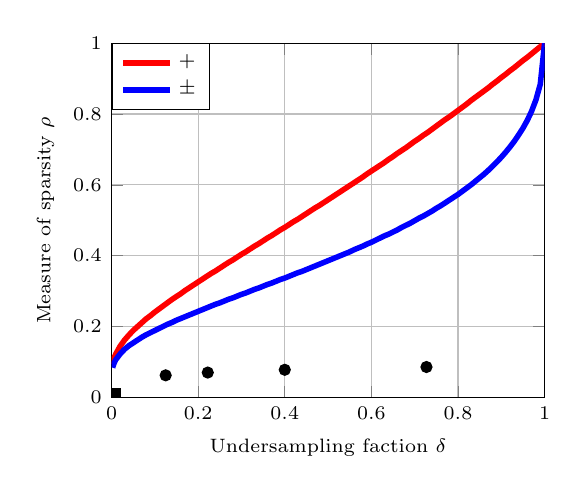
\begin{tikzpicture}

\begin{axis}[%
font=\scriptsize,
width=5.5cm,
height=4.5cm,
scale only axis,
xmin=0,
xmax=1,
xlabel={Undersampling faction $\delta$},
xmajorgrids,
ymin=0,
ymax=1,
ylabel={Measure of sparsity $\rho$},
%ylabel near ticks,
ymajorgrids,
legend style={at={(0,1)},anchor=north west,legend cell align=left,
/tikz/column 2/.style={column sep=3pt}}
]

\addplot [color=red,solid,line width=2.0pt]
  coordinates {
(0.0025,0.094) (0.005,0.107) (0.0075,0.116)
(0.01,0.123) (0.02,0.145) (0.03,0.162) (0.04,0.176) (0.05,0.189) (0.06,0.2) (0.07,0.211) (0.08,0.222) (0.09,0.231) (0.1,0.241) (0.11,0.25) (0.12,0.259) (0.13,0.268) (0.14,0.277) (0.15,0.285) (0.16,0.293) (0.17,0.302) (0.18,0.31) (0.19,0.318) (0.2,0.326) (0.21,0.334) (0.22,0.342) (0.23,0.35) (0.24,0.357) (0.25,0.365) (0.26,0.373) (0.27,0.381) (0.28,0.388) (0.29,0.396) (0.3,0.404) (0.31,0.411) (0.32,0.419) (0.33,0.427) (0.34,0.434) (0.35,0.442) (0.36,0.45) (0.37,0.457) (0.38,0.465) (0.39,0.473) (0.4,0.48) (0.41,0.488) (0.42,0.496) (0.43,0.503) (0.44,0.511) (0.45,0.519) (0.46,0.527) (0.47,0.535) (0.48,0.542) (0.49,0.55) (0.5,0.558) (0.51,0.566) (0.52,0.574) (0.53,0.582) (0.54,0.59) (0.55,0.598) (0.56,0.606) (0.57,0.614) (0.58,0.622) (0.59,0.631) (0.6,0.639) (0.61,0.647) (0.62,0.655) (0.63,0.663) (0.64,0.672) (0.65,0.68) (0.66,0.689) (0.67,0.697) (0.68,0.705) (0.69,0.714) (0.7,0.723) (0.71,0.731) (0.72,0.74) (0.73,0.748) (0.74,0.757) (0.75,0.766) (0.76,0.775) (0.77,0.784) (0.78,0.792) (0.79,0.801) (0.8,0.81) (0.81,0.819) (0.82,0.828) (0.83,0.838) (0.84,0.847) (0.85,0.856) (0.86,0.865) (0.87,0.874) (0.88,0.884) (0.89,0.893) (0.9,0.903) (0.91,0.912) (0.92,0.922) (0.93,0.931) (0.94,0.941) (0.95,0.951) (0.96,0.96) (0.97,0.97) (0.98,0.98) (0.99,0.99) (1,1)
};
\addlegendentry{$+$};

\addplot [color=blue,solid,line width=2.0pt]
  coordinates {
(0.0025,0.084) (0.005,0.094) (0.0075,0.101)
(0.01,0.107) (0.02,0.123) (0.03,0.136) (0.04,0.146) (0.05,0.154) (0.06,0.162) (0.07,0.17) (0.08,0.177) (0.09,0.183) (0.1,0.189) (0.11,0.195) (0.12,0.201) (0.13,0.207) (0.14,0.212) (0.15,0.218) (0.16,0.223) (0.17,0.228) (0.18,0.233) (0.19,0.238) (0.2,0.243) (0.21,0.248) (0.22,0.253) (0.23,0.258) (0.24,0.263) (0.25,0.267) (0.26,0.272) (0.27,0.277) (0.28,0.281) (0.29,0.286) (0.3,0.291) (0.31,0.295) (0.32,0.3) (0.33,0.305) (0.34,0.309) (0.35,0.314) (0.36,0.319) (0.37,0.323) (0.38,0.328) (0.39,0.333) (0.4,0.337) (0.41,0.342) (0.42,0.347) (0.43,0.352) (0.44,0.356) (0.45,0.361) (0.46,0.366) (0.47,0.371) (0.48,0.376) (0.49,0.381) (0.5,0.386) (0.51,0.391) (0.52,0.396) (0.53,0.401) (0.54,0.406) (0.55,0.411) (0.56,0.417) (0.57,0.422) (0.58,0.427) (0.59,0.433) (0.6,0.438) (0.61,0.444) (0.62,0.45) (0.63,0.456) (0.64,0.461) (0.65,0.467) (0.66,0.473) (0.67,0.48) (0.68,0.486) (0.69,0.492) (0.7,0.499) (0.71,0.506) (0.72,0.512) (0.73,0.519) (0.74,0.526) (0.75,0.534) (0.76,0.541) (0.77,0.549) (0.78,0.557) (0.79,0.565) (0.8,0.573) (0.81,0.582) (0.82,0.591) (0.83,0.6) (0.84,0.61) (0.85,0.62) (0.86,0.63) (0.87,0.641) (0.88,0.653) (0.89,0.665) (0.9,0.678) (0.91,0.692) (0.92,0.707) (0.93,0.723) (0.94,0.741) (0.95,0.76) (0.96,0.782) (0.97,0.808) (0.98,0.84) (0.99,0.884) (1,1)
};
\addlegendentry{$\pm$};

%\node at (axis cs: 0.2, 0.65) {Failure Region};
%\node at (axis cs: 0.685, 0.25) {Exact Reconstruction};

\filldraw [fill=black] (axis cs:0,0) rectangle (axis cs:0.02,0.025);

\filldraw (axis cs: 0.125, 0.0625) circle (2pt);
\filldraw (axis cs: 0.2222,0.0703125) circle (2pt);
\filldraw (axis cs: 0.4, 0.078125) circle (2pt);
\filldraw (axis cs: 0.7272,0.0859375) circle (2pt);

%\filldraw[color=darkgray] (axis cs: 0.000001, 0.0625) circle (1.5pt);
%\filldraw[color=darkgray] (axis cs: 0.000006, 0.0703125) circle (1.5pt);
%\filldraw[color=darkgray] (axis cs: 0.00004, 0.078125) circle (1.5pt);
%\filldraw[color=darkgray] (axis cs: 0.00018, 0.0859375) circle (1.5pt);
%\filldraw[color=darkgray] (axis cs: 0.00065, 0.09375) circle (1.5pt);
%\filldraw[color=darkgray] (axis cs: 0.00240, 0.1015625) circle (1.5pt);
%\filldraw[color=darkgray] (axis cs: 0.00446, 0.109375) circle (1.5pt);
%\filldraw[color=darkgray] (axis cs: 0.00833, 0.1171875) circle (1.5pt);
%\filldraw[color=darkgray] (axis cs: 0.03125, 0.125) circle (1.5pt);
%\filldraw[color=darkgray] (axis cs: 0.055555, 0.140625) circle (1.5pt);
%\filldraw[color=darkgray] (axis cs: 0.2, 0.15625) circle (1.5pt);
\end{axis}

\end{tikzpicture}
